%%%% CAPÍTULO 3 - MATERIAL E MÉTODOS (PODE SER OUTRO TÍTULO DE ACORDO COM O TRABALHO REALIZADO)

\chapter{Metodologia}\label{cap:metodologia}


Esta seção apresenta a metodologia aplicada na investigação, sobre como como LLMs podem aprender, ou como se diferenciam nesta representação, da tarefa de solução de labirintos em ASCII, por meio da análise das mudanças nas ativações internas das redes neurais, após diferentes estratégias de \textit{fine-tuning}. O objetivo desta seção é detalhar os procedimentos adotados, de modo a garantir a replicabilidade do estudo, incluindo preparação dos dados, modelos, métricas e análises estatísticas utilizadas.

\section{Dados}

Foram utilizadas amostras do conjunto de dados de treino, disponibilizado por \citet{dao2025alphamaze}, representados em ASCII, uma vez que esses dados estão disponíveis publicamente e permitiram uma redução considerável no tempo que seria empregado na elaboração dos datasets e ajuste dos modelos.

\begin{itemize}
    \item \textbf{Formato geral dos exemplos}: cada exemplo é um \textit{prompt} textual que instrui o modelo sobre a tarefa, apresenta a grade completa do labirinto com origem e destino e define que a saída deve conter apenas tokens de movimento.

    \item \textbf{Tokenização do labirinto}: a descrição é composta por tokens delimitados no padrão \verb!<|...|>!, incluindo:
    \begin{itemize}
        \item \textit{Coordenadas}: \verb!<|row-col|>! (ex.: \verb!<|0-0|>!, \verb!<|3-2|>!) indicam a posição absoluta da célula na grade.
        \item \textit{Paredes}: um único token resume as paredes presentes na célula, combinando direções com \textit{underscore} (\_), por exemplo \verb!<|up_wall|>!, \verb!<|left_right_wall|>!, \verb!<|up_left_right_wall|>! que indicam a existência de paredes acima, à esquerda e à direita e acima, esquerda e direita, respectivamente.
        \item \textit{Marcadores especiais}: \verb!<|origin|>!, indica a origem (ponto de partida) e \verb!<|target|>! indica o destino final (ponto de chegada) do labirinto.
        \item \textit{Separador}: \verb!<|blank|>! atua como espaçamento explícito entre grupos de tokens/células, reduzindo ambiguidade de fronteiras.
        \item \textit{Vocabulário de movimentos} (saída do modelo): tokens que os modelos devem utilizar para descrever a sua resposta, sendo eles, \verb!<|up|>!, \verb!<|down|>!, \verb!<|left|>!, \verb!<|right|>! que representam movimentos para cima, para baixo, para a esquerda e para a direita, respectivamente.
    \end{itemize}

    \item \textbf{Padrão por célula}: cada célula descrita em uma solicitação segue tipicamente o padrão \verb!<|row-col|><|wall_pattern|><|blank|>!, com este último podendo incluir \verb!<|origin|>! ou \verb!<|target|>!, quando aplicável.
    
    \item \textbf{Formato da resposta}: o modelo deve emitir apenas a sequência de tokens de movimento, separados por espaços, que leva da origem (\verb!<|origin|>!) ao destino (\verb!<|target|>!). Nos prompts, incentiva-se, como diretriz adicional para melhor resolução de problemas, a ação ``think step-by-step'' (``\textit{pense passo a passo}''), em tradução livre. Entretanto, de qualquer forma, a saída final deve conter exclusivamente os tokens de movimento, conforme especificado anteriormente.
\end{itemize}

A \autoref{fig:exemplo-prompt} ilustra um dos prompts presentes no dataset empregado, proveniente do trabalho de \citet{dao2025alphamaze}. Na parte inferior da figura, é apresentado um exemplo do labirinto em formato ASCII, conforme o padrão anteriormente descrito.

\begin{figure}[h!]
    \centering
    \caption{Exemplo de solicitação (\textit{prompt}) trabalhados.}
    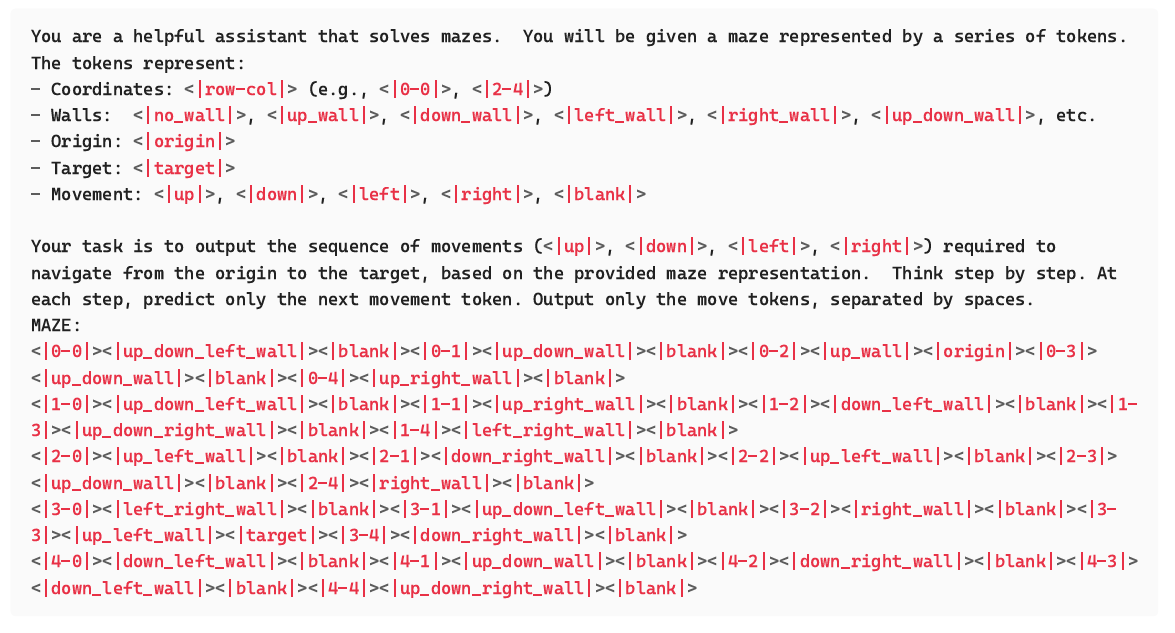
\includegraphics[width=0.75\textwidth]{figuras/exemplo-prompt.png}
    \label{fig:exemplo-prompt}
    \fonte{}
\end{figure}

Ressalta-se, como diretriz metodológica, que embora o \textit{dataset} reaproveitado inclua a sequência de passos da resposta correta e o trabalho de \citet{dao2025alphamaze} avalie a acurácia e o desempenho dos modelos na resolução dos labirintos, tais informações externas de acertos não foram utilizadas como métrica neste estudo. O foco desta investigação restringe-se às dinâmicas das ativações internas, independentemente do sucesso final da navegação.

\section{Modelos e Estratégias de Fine-tuning}

Foram selecionados três LLMs, todos com 1,5B de parâmetros, compatíveis com a biblioteca LLM-MRI, obtidos via Hugging Face Hub \cite{hf-hugging-face-hub-2025}. Informações gerais acerca dos modelos são apresentados na \autoref{tab:modelos-utilizados}.
\begin{table}[h!]
    \centering
    \caption{Informações dos modelos utilizados nos experimentos}
    \label{tab:modelos-utilizados}
    \begin{tabular}{|l|l|c|l|}
        \hline
        \textbf{Nome} & \textbf{Tipo Ajuste} & \textbf{Parâmetros} & \textbf{Licença} \\
        \hline
        DeepSeek-R1-Distill-Qwen-1.5B & Base & 1.5B & MIT \\
        AlphaMaze-v0.2-1.5B-SFT & SFT & 1.5B & Apache-2.0 \\
        AlphaMaze-v0.2-1.5B & GRPO & 1.5B & Apache-2.0 \\
        \hline
    \end{tabular}
    \fonte{}
\end{table}

\begin{itemize}
    \item \textbf{DeepSeek-R1-Distill-Qwen-1.5B} (\cite{hf-deepseek-r1-dq-1p5b}): modelo denso destilado a partir do DeepSeek-R1 sobre a família Qwen2.5, utilizado como ponto de partida antes de ajustes específicos \cite{hf-deepseek-r1-dq-1p5b}.
    \item \textbf{AlphaMaze-v0.2-1.5B-SFT} (\cite{hf-jan-alpha-sft-1p5b}): variante ajustada por SFT, empregada para avaliar o impacto do ajuste supervisionado na tarefa de labirintos \cite{hf-jan-alpha-sft-1p5b}.
    \item \textbf{AlphaMaze-v0.2-1.5B} (\cite{hf-menlo-alphamaze-v02-1p5b}): variante ajustada por GRPO, usada para comparar a dinâmica de aprendizado por otimização de política relativa a preferências \cite{hf-menlo-alphamaze-v02-1p5b, dao2025alphamaze}.
\end{itemize}

De acordo com \citet{dao2025alphamaze}, cada modelo foi treinado separadamente em cada estratégia, com conjuntos de dados de treino específicos para o modelo ajustado com SFT e para o modelo ajustado com GRPO, em que seu conjunto de dados de treino possui orientações adicionais para potencializar sua autocorreção conforme a otimização política relativa a preferências. Ambos os modelos ajustados compartilham a mesma arquitetura e número de parâmetros do modelo base DeepSeek-R1-Distill-Qwen-1.5B. Desta forma, foi reaproveitado todo o processo de treinamento e especialização dos modelos, com diferentes estratégias de \textit{fine-tuning}, conforme discutido na literatura que estão descritas a seguir:

\begin{itemize}
    \item \textbf{Supervised Fine-Tuning (SFT)}: ajuste supervisionado utilizando exemplos de labirintos e suas soluções.
    \item \textbf{Group Relative Policy Optimization (GRPO)}: ajuste baseado em preferências coletivas, visando aprimorar o raciocínio e a autocorreção dos modelos.
\end{itemize}

Para contextualizar a capacidade de raciocínio espacial dos modelos selecionados, é relevante observar o desempenho original reportado pelos autores do AlphaMaze. Conforme demonstrado na Tabela \autoref{tab:desempenho-mazebench}, o modelo base (DeepSeek-R1-Distill-Qwen-1.5B) não foi capaz de resolver nenhum dos labirintos do \textit{benchmark}, apresentando acurácia nula. A aplicação do Supervised Fine-Tuning (SFT) elevou drasticamente essa capacidade para 86,0\%, estabelecendo uma competência fundamental de navegação. Por fim, o refino via Group Relative Policy Optimization (GRPO) permitiu ao modelo alcançar 93,0\% de acurácia, indicando uma sofisticação no processo de decisão sequencial e autocorreção \cite{dao2025alphamaze}.

\begin{table}[h!]
    \centering
    \caption{Acurácia de resolução de labirintos no \textit{MazeBench}}
    \label{tab:desempenho-mazebench}
    \begin{tabular}{|l|c|c|r|}
        \hline
        \textbf{Modelo} & \textbf{SFT} & \textbf{GRPO} & \textbf{Score (\%)} \\
        \hline
        DeepSeek-R1-Distill-Qwen-1.5B (Base) & Não & Não & 0,0 \\
        AlphaMaze-v0.2-1.5B-SFT & Sim & Não & 86,0 \\
        AlphaMaze-v0.2-1.5B (GRPO) & Sim & Não & \textbf{93,0} \\
        \hline
    \end{tabular}
    \fonte{\citet{dao2025alphamaze}}
\end{table}

\section{Procedimentos de Processamento, Métricas e Estatística}

A obtenção das ativações internas dos modelos foi feita com a utilização da biblioteca LLM-MRI \cite{costa2024llmmri}, que permite, além da extração, a visualização das ativações neuronais de LLMs. Portanto, aqui estão descritos os procedimentos adotados para o processamento dos dados e a extração das ativações, bem como as análises estatísticas subsequentes.

\subsection{Pré-processamento e Validação Inicial}

O pré-processamento dos dados envolveu as etapas descritas a seguir.
\begin{itemize}
    \item Obtenção dos arquivos Parquet do \textit{dataset} de treinamento do modelo AlphaMaze-v0.2-1.5B-SFT, contendo os prompts e as respostas geradas pelos modelos.
    \item Atribuição de \textit{label} binária (\textit{easy} = 0, \textit{complex} = 1) por um limiar de passos ($<10$ passos, \textit{easy}; \textit{complex}, caso contrário) para se adequar a análises categóricas, necessário para utilizar a biblioteca LLM-MRI.
    \item Validação de \textit{embbeddings} extraídos dos modelos pela biblioteca LLM-MRI com modelos de aprendizado de máquina de regressão logística. Validação realizada antes e depois da aplicação da redução de dimensionalidade para assegurar a consistência do funcionamento da biblioteca. De acordo com os resulados obtidos na validação dos \textit{embeddings}, foi possível confirmar o funcionamento adequado da biblioteca LLM-MRI para extração das ativações dos modelos selecionados. Sendo que para o resultado do modelo de regressão logística aplicado sobre os \textit{embeddings} antes da redução de dimensionalidade, obteve-se uma acurácia de 100\%.
\end{itemize}

\subsection{Métricas de Ciências das Redes}\label{sec:metodologia-metricas}

As métricas de ciências das redes utilizadas para caracterizar os grafos de ativações para as camada dos modelos estão descritas a seguir. Os grafos utilizados foram construídos conforme a LLM-MRI. As métricas dependentes de caminhos foram calculadas sobre a maior componente conexa (Largest Connected Component - LCC).

\begin{itemize}
    \item \textbf{Número de Nós} ($|V|$): número total de nós (ordem) do grafo.
    \item \textbf{Número de Arestas} ($|E|$): número total de arestas do grafo.
    \item \textbf{Grau Médio} ($\bar{k}$): média do grau dos nós.
    \item \textbf{Densidade} ($\rho$): fração de arestas observadas em relação ao máximo possível. Valores mais altos indicam conectividade mais densa.
    \item \textbf{Assortatividade} ($r$): coeficiente de assortatividade. Valores positivos indicam tendência de nós de alto grau conectarem-se entre si; negativos indicam conexões preferenciais entre nós de alto e baixo grau.
    \item \textbf{Diâmetro} ($D$): maior distância entre pares de nós na LCC do grafo, isto é, comprimento do caminho mais curto máximo. Quando o grafo não é totalmente conexo, $D$ é calculado na LCC.
    \item \textbf{Comprimento Médio de Caminho} ($\bar{L}$): distância média entre todos os pares de nós na LCC.
\end{itemize}

\subsection{Amostragem para Inferência de Distribuições}

Empregou-se um protocolo de amostragem repetida para estimar a variabilidade das métricas de rede, sem amostragem repetida de prompts em um mesmo experimento. Em cada experimento modelos foram comparados sob entradas idênticas.

Em cada experimento, foram selecionados 40 prompts distintos (sem reposição) e foi repetido o procedimento em 1000 experimentos, mantendo o mesmo lote (40 prompts) por experimento entre os três modelos. Além disso, foi realizado uma segunda bateria de 1000 experimentos, neste caso, considerando os dados do grafo das ativações apenas das últimas cinco camadas, para investigar o efeito do fine-tunning nas camadas mais especializadas. Os passos por experimento estão descritos com maior detalhamento a seguir.

\begin{enumerate}
    \item Selecionou-se um lote de 40 prompts;
    \item Coletaram-se as ativações em cada modelo via LLM-MRI;
    \item Obteve-se o grafo das ativações;
    \item Calcularam-se as métricas mencionadas anteriormente.
    \item Registrou-se as métricas e o tempo total de processamento por experimento e modelo.
\end{enumerate}

Sementes pseudoaleatorias foram fixadas para reprodutibilidade, bem como versões de bibliotecas foram anotadas. Para cada métrica e modelo, foram gerados: histogramas; estimativas de densidade por núcleo (\textit{Kernel Density Estimation} -- KDE) e curvas de média cumulativa por índice de experimento, visando inspecionar estabilização. Este mesmo procedimento foi replicado para a configuração de ``todas as camadas'' e para ``últimas cinco camadas'' de ativações.

\subsection{Significância Estatística}

Ao término do procedimento de amostragem, foram realizados testes de significância estatística entre as distribuições das métricas de rede dos três modelos, para as duas configurações especificadas (todas as camadas e últimas cinco camadas). Inicialmente, foi aplicado o teste ANOVA de uma via para verificar a existência de diferenças globais entre as distribuições das métricas dos três modelos. Em seguida, foram realizados testes t pareados entre os pares de modelos (Base vs SFT e Base vs GRPO) para identificar quais pares apresentavam diferenças estatisticamente significativas. As hipóteses estabelecidas para essa verificação estatística estão descritas a seguir.

\begin{itemize}
\item \textbf{Hipótese nula (H0)}: as distribuições de cada métrica são equivalentes entre os modelos comparados.
\item \textbf{Hipótese alternativa (H1)}: existe diferença estatisticamente significativa entre pelo menos dois modelos para a métrica analisada.
\end{itemize}


\section{Máquina e Recursos Computacionais}
\label{sec:ambiente-maquina}

Os experimentos foram executados em uma única máquina, utilizando exclusivamente o processador (CPU) do equipamento, embora uma GPU estivesse disponível e funcional no sistema, não foi necessária a sua utilização nos procedimentos descritos neste trabalho. Os tempos reportados referem-se ao tempo de processamento medido por experimento, registrados durante a extração das ativações via LLM-MRI e o cálculo das métricas de rede.

\subsection{Tempos de Execução}

\begin{itemize}
    \item Duração total (1000 experimentos para todas as camadas): \textbf{64,24 horas}.
    \item Duração média por experimento (todas as camadas): \textbf{77,09 segundos}.
    \item Duração total (1000 experimentos para últimas 5 camadas): \textbf{88,68 horas}.
    \item Duração média por experimento (últimas 5 camadas): \textbf{106,42 segundos}.
\end{itemize}

\subsection{Configuração da máquina}

As informações a seguir foram obtidas a partir do gerenciador de tarefas do Windows (captura de configuração e métricas no momento da execução/registro):

\begin{itemize}
    \item \textbf{CPU}: 13th Gen Intel(R) Core(TM) i7-13700HX (Velocidade base: 2,10 GHz; Núcleos: 16; Processadores lógicos: 24).
    \item \textbf{Memória (RAM)}: 16,0 GB (SODIMM, 4800 MT/s; 2 de 4 slots usados).
    \item \textbf{GPU (disponível, não utilizada)}: NVIDIA GeForce RTX 4050 Laptop GPU; Memória dedicada da GPU: 6,0 GB.
    \item \textbf{Armazenamento:} SSD NVMe (477 GB).
\end{itemize}

\section{Síntese Metodológica e Hipóteses Iniciais}

Os procedimentos descritos nesta seção estabelecem o fluxo experimental aplicado para investigar como diferentes estratégias de \textit{fine-tuning} impactam as ativações internas de LLMs na tarefa de solução de labirintos em ASCII. Com a aplicação dessa metodologia, serão examinadas as seguintes hipóteses:

\begin{itemize}
    \item[H1:] Estratégias distintas de \textit{fine-tuning} (SFT e GRPO) induzem padrões diferentes de ativação interna, refletindo abordagens variadas de raciocínio espacial e de representação da tarefa.
    \item[H2:] A análise das ativações neuronais por meio da LLM-MRI permite identificar alterações estruturais e padrões emergentes associados ao aprendizado da tarefa, contribuindo para a compreensão dos mecanismos internos dos modelos.
\end{itemize}

Na seção seguinte, estão apresentados os resultados para embasar a discussão sobre as hipóteses formuladas.
